\documentclass[10pt,foldmark,notumble]{leaflet}
\usepackage[ngerman]{babel}
\usepackage[utf8]{inputenc} % ueoeaess
\usepackage{enumitem}% http://ctan.org/pkg/enumitem

\usepackage{csquotes}
\MakeOuterQuote{"}

\usepackage{titlesec}
%\titlespacing*{<command>}{<left>}{<before-sep>}{<after-sep>}
\titlespacing*{\section   }{0pt}{7pt}{0pt}
\titlespacing*{\subsection}{0pt}{5pt}{0pt}

\usepackage{xcolor}


\renewcommand*\foldmarkrule{.3mm}
%\renewcommand*\foldmarklength{5mm}

\begin{document}

    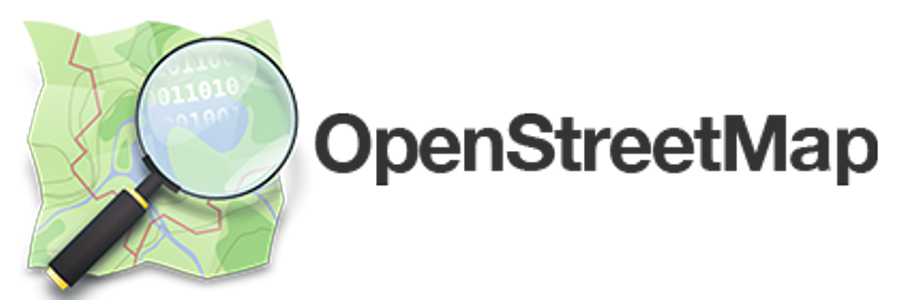
\includegraphics[width=\linewidth]{logo.png}

    \section{Unterwegs für eine freie Weltkarte}
    Hallo!

    Wenn Sie das lesen, haben Sie mich wahrscheinlich angesprochen, weil Sie wissen möchten, was ich hier in Ihrem Wohngebiet tue.

    Ich erhebe hier Daten für "OpenStreetMap", was das ist erfahren Sie auf der Innenseite.

    Aber wenn Sie's ganz eilig haben:
    \begin{itemize}[noitemsep,topsep=0pt]
        \item Nein, ich tue hier nichts schlimmes {\small(im Gegenteil, es ist gemeinnützige Arbeit!)}
        \item Nein, was ich hier tue ist nicht illegal
        \item Ihnen entsteht kein Schaden durch das, was ich hier tue {\small(im Gegenteil, es könnte Ihnen helfen!)}
        \item Nein, ich spioniere nicht Ihr Haus aus, um später einzubrechen :D
    \end{itemize}
    Wenn Ihnen das reicht: Gern geschehen!

    Wenn Sie weitere Fragen haben oder mehr über das Projekt wissen wollen, lesen Sie gerne im inneren dieses Flyers weiter! :)

    \section{Was ist OpenStreetMap?}
    Eine sehr einfache Erklärung, die in der Community sehr beliebt ist, ist: "Kennen Sie Google Maps? Ja, das ist sowas ähnliches." Und diese Erklärung ist auch richtig und in den meisten Fällen zutreffend, allerdings halte ich sie für unnötig vereinfachend, denn sie verkennt eine wichtige Eigenschaft des Projektes. Wenn Sie auf osm.org gehen, sehen Sie eine Karte, die viele Leute für "die" OpenStreetMap halten. Und Sie werden die Karte vielleicht ansehen und sagen "Aber Moment, eine Straße sieht doch immer gleich aus. Wenn man einträgt, ob eine Straße einen Bürgersteig hat, sieht man das auf der Karte doch gar nicht!" Exakt. 99\% der Daten, die ich hier erhebe, werden nicht auf dieser Karte dargestellt. OpenStreetMap ist nämlich nicht "diese Karte", sondern eine Bezeichnung für die Datenbank mit Infos über unzählige Objekte in der realen Welt. Ich beschreibe es gerne als "Wikipedia für Dinge mit Koordinaten". Jemand, der eine Karte erstellt, entscheidet dann, welche Daten wie auf seiner Karte zu sehen sind und welche nicht. Gehen Sie zum Beispiel auf opencyclemap.org, so sehen Sie eine Karte, auf der für Radfahrer besonders wichtige Informationen hervorgehoben sind, wie Radwanderwege, Unterstände und Fahrradgeschäfte. Diese Karte basiert auf denselben Daten wie die andere, nur werden sie anders Dargestellt. Feuerwehren zum Beispiel nutzen auch Karten, die auf genau dieser Datenbank basieren, nur sind auf deren Karten Hydranten sichtbar. Und auch viele humanitäre Zwecke profitieren von OpenStreetMap-Daten. Auf wheelmap.org finden Sie z.B. eine Karte, die die Bedürfnisse von Rollstuhlfahrern in den Vordergrund stellt. Und einem Blinden kann eine spezielle App mithilfe von OpenStreetMap-Daten sagen, wo er langlaufen muss, um nur an Ampeln mit Blindenhilfe vorbeizukommen.

    Ich bearbeite also gar nicht wirklich "die Karte", sondern befülle eine Datenbank mit Fakten über die echte Welt, aus der dann jeder (auch Sie, wenn Sie wollen!) sich Karten, Apps und Stadtpläne nach seinen Wünschen generieren kann.

    Sollten Sie das jetzt aber alles zu verwirrend oder zu kompliziert finden, keine Sorge. Am Ende ist auch die Aussage "Es ist wie Google Maps." vollkommen ausreichend.

    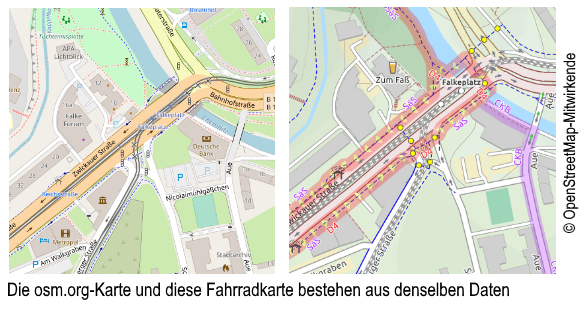
\includegraphics[width=\linewidth]{karte.png}


    \section{Wieso OpenStreetMap statt z.B. Google Maps?}
    \subsection{Zunächst das offensichtliche Vorweg:}
    OpenStreetMap ist ein gemeinfreies Projekt. Es gehört keinem Großkonzern wie Google, deswegen wertet auch niemand aus, was Sie sich auf osm.org ansehen, oder welche Routen sie planen und versucht dann Ihnen entsprechende Werbung zu zeigen.

    \subsection{Zum anderen: Qualität!}
    Daten von OSM sind in vielen Punkten
    \begin{itemize}[noitemsep,topsep=0pt]
        \item genauer
        \item aktueller und
        \item umfangreicher
    \end{itemize}
    als z.B. von Google Maps.

    \begin{itemize}[noitemsep,topsep=0pt]
        \item Google Maps kennt Straßen, OSM kennt Trampelpfade, Hinterhofwege und Wege in öffentlichen Gebäuden.
        \item Google weiß, das hier eine Straße ist. OSM weiß, ob sie einen Bürgersteig hat, ob sie nachts beleuchtet ist, welchen Straßenbelag sie hat, welche Höchstgeschwindigkeit sie hat und vieles mehr.
        \item Google Maps kennt in einem Park Gehwege, OSM kennt Aussichtspunkte, Sitzbänke, Mülleimer, Hundekottütenspender und teilweise jeden einzelnen Baum.
        \item Google Maps bietet die beste Navigation -- für Autofahrer. Sobald Sie mit dem Fahrrad oder zu Fuß unterwegs sind, sind sie ohne eine App, die OSM-Daten nutzt, komplett verlassen
        \item Schaukelt das Kind gerne? Google kennt -- wenn Sie Glück haben -- Spielplätze. OSM weiß, was für Spielgeräte auf welchen Spielplätzen stehen.
    \end{itemize}

    \subsection{Als letztes: Freiheit}
    Mein Hauptgrund als Informatiker und Programmierer OSM zu nutzen ist, dass Google viele Daten gar nicht oder nur gegen viel Geld herausgibt. OpenStreetMap-Daten sind nicht nur kostenlos, sondern dürfen für jeden Zweck verwendet werden! Solange Sie kenntlich machen, dass es sich um OSM-Daten handelt, dürfen Sie die Daten zu jedem Zweck verwenden, sogar kommerziell.

    Sie wollen das Buch "Der deutsche Döneratlas" herausbringen und damit millionen scheffeln? Mit Google dürften und könnten Sie das nicht. Mit OSM schon!


    \section{Häufig gestellte Fragen}
    \subsection{Welche Daten erheben Sie?}
    Mit der App, mit der ich meistens arbeite, erhebe ich ca. 100 verschiedene Datentypen. Sie finden auf der rechten Seite eine Auflistung. Allerdings mache ich manchmal auch Fotos von Dingen, die ich mit meiner App nicht verzeichnen kann, und trage sie später per Hand ein.

    \subsection{In wessen Auftrag erheben Sie die Daten?}
    Niemand hat mir "den Auftrag" gegeben, das zu tun. Ich tue es in meiner Freizeit, weil ich es möchte.

    \subsection{Werden Sie für das Erheben der Daten bezahlt?}
    Nein, ich mache das unentgeldlich in meiner Freizeit.

    \subsection{Werden die Daten verkauft?}
    Nein. Die gesamte OpenStreetMap-Datenbank ist kostenlos für jeden verfügbar. Die Daten zu "verkaufen" wäre zwar erlaubt, aber wer würde sie kaufen, wenn sie doch kostenlos zur verfügung stehen?

    \subsection{Wer hat Zugriff auf diese Daten?}
    Wie gesagt, die Datenbank ist kostenlos für jeden im Internet abrufbar. Also lautet die Antwort: jeder auf der Welt.


    \section{Häufig gestellte Fragen {\small ... aber als Anschuldigungen formuliert}}
    \subsection{Daten über mein Haus sind personenbezogene Daten, die Sie ohne mein Einverständnis nicht erheben dürfen!}
    Doch. Die Infos, die ich erhebe, sind sog. "nicht schützenswerte Daten". Ein Datenpunkt, der unter diese Schutzwürdigkeit fällt, wäre z.B. Wer in einem Haus wohnt. So etwas dürfte ich nicht (und möchte ich auch nicht) erheben.

    \subsection{Sie haben Fotos von meinem Grundstück gemacht, das dürfen Sie nicht!}
    Obwohl dieser Flyer lange vor meinem Aushändigen an Sie geschrieben wurde, kann ich Ihnen versichern, dass ich kein(e) Foto(s) von Ihnen oder Ihrem Grundstück gemacht habe. Danach habe ich weder ein Bedürfnis noch habe ich Speicherplatz dafür. Wie gesagt mache ich manchmal Fotos von Objekten wie Briefkästen (also Postbriefkästen! Nicht die an Häusern) oder Spielplätzen, um sie später per Hand einzutragen. Es handelt sich also höchstwahrscheinlich um ein Missverständnis. Aber nur nebenbei: Ich dürfte es, wenn ich wollte. Es gibt zwar ein Recht am eigenen Bild, aber kein Recht am Bild des eigenen Eigentums.

    \subsection{Wenn Sie Daten erheben, muss es einen Ansprechpartner geben, wer ist das?}
    Bei OpenStreetMap gibt es keinen offiziellen Ansprechpartner. Die Datenbank wird rechtlich gesehen von der Openstreetmap-Foundation betrieben, deren "local Chapter" für Deutschland der FOSSGIS e.V. ist. Aber der ist trotzdem kein guter Ansprechpartner, um sich über meine Erhebung hier zu beschweren, da ich kein Mitglied dieses Vereins bin.


    \subsection{Daten, die ich erhebe:}
    \begin{itemize}[noitemsep,topsep=0pt]
        \item Ob Straßen, Wege, Bushaltestellen und Sportplätze nachts beleuchtet sind
        \item Straßennamen, Hausnummern, zu welchen Straßen Häuser gehören
        \item Gebäudetypen, Anzahl der Geschosse und Dachgeschosse, Dachformen
        \item Wann Briefkästen geleert werden
        \item Ob Einrichtungen wie Sitzbänke, Telefone, Automaten und Infotafeln noch existieren
        \item Ob Straßen einen Bürgersteig haben und wenn ja auf welchen Seiten
        \item Ob Straßen Radwege haben, und wenn ja was für welche auf welchen Seiten
        \item Ob Baustellen bereits abgeschlossen sind
        \item Recyclingmöglichkeiten: Was für eine Art, ob jede Art von Glas oder nur Flaschen und Gläser entsorgt werden dürfen, was dort entsorgt werden kann
        \item Welche Oberfläche Straßen und Wege haben
        \item Welche Höchstgeschwindigkeit, Maximalgewicht und Maximalhöhe auf einer Straße gilt
        \item Wie viele Fahrstreifen in welche Richtung eine Straße hat
        \item Öffnungszeiten
        \item An Ampeln und Fußgängerüberwegen: Ob es eine Verkehrsinsel gibt, ob eine Ampel akustische Signale oder einen Taster für Sehbehinderte hat, ob es eine Bedarfsampel ist
        \item Bushaltestellen: Ob sie einen Unterstand und eine Bank haben und ob es Blindenpflasterung gibt
        \item Ob Restaurants vegetarische und vegane Speisen anbieten
        \item Parkplätze: Ob sie Privat-, öffentliche oder Kundenparkplätze sind, ob sie Gebühr kosten und was für Parkplätze es sind
        \item Ob Orte für Rollstühle zugänglich sind, ob Toiletten für Rollstühle zugänglich sind
        \item Ob Spielplätze für die öffentlichkeit Zugänglich sind
        \item Treppen: Welche Richtung führt nach oben? Gibt es ein Geländer? Gibt es eine Rampe? Stufenanzahl?
        \item Ob Sitzbänke eine Rückenlehne haben, Hydrantentypen
        \item Wer ist Betreiber von Altkleidercontainern, Geldautomaten und E-Auto-Ladestationen?
    \end{itemize}


    \vfill
    \textcolor{gray}{\small Dieser Flyer wurde vom OSM-User wielandb erstellt und steht unter CC-BY 2.0. Er darf frei kopiert, weitergegeben und verändert werden, solange dieser Hinweis bestehen bleibt. Version 1.6}

\end{document}
